\documentclass[12pt]{article}

\usepackage{sbc-template}

\usepackage{graphicx,url}
\usepackage{subfigure}

\usepackage[brazil]{babel}   
\usepackage[latin1]{inputenc}  
     
\sloppy

\title{MI - Concorr�ncia e Conectividade\\}

\author{Wanderson Bezerra e Vinicius Pereira Santana}

\address{Graduando em Engenharia de Computa��o. \\ Universidade Estadual de Feira de Santana (UEFS), Feira de Santana, Brasil.
  \email{-}
}

\begin{document} 

\maketitle

\begin{abstract}
  
\end{abstract}
     
\begin{resumo} 

\end{resumo}


\section{Introdu��o}

%\begin{figure}[h]
%	
%	\center
%	\subfigure[tela\_inicial][Tela Inicial.]{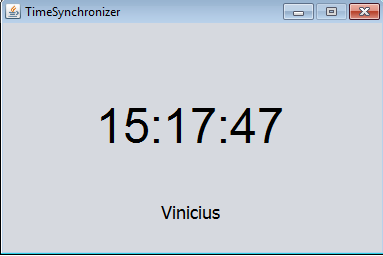
\includegraphics[scale = 0.45]{tela_inicial.eps}}
%	\qquad
%	\subfigure[home\_page][Home-Page com as opera��es dispon�veis.]{\includegraphics[scale = 0.45]{home_cliente.eps}}
%	\caption{Imagens do sistema desenvolvido.}
%	\label{sistemaimgs}
%	
%\end{figure}


\section{Conclus�es}\label{concl}


\bibliographystyle{sbc}
\bibliography{sbc-template}

\end{document}
